% -*- coding: utf-8 -*-
\section{Introduction}
\label{sec:intro}
The finite-difference time-domain\index{finite-difference time-domain} (FDTD\index{FDTD}) method is a numerical algorithm which calculates the time-evolution of the electromagnetic fields by solving Maxwell's equations\index{Maxwell's equations}. The FDTD\index{FDTD} algorithm requires relatively less constraints compared to other numerical methods, and hence has been widely adopted in various design problems in the areas of electromagnetics and photonics \cite{taflove_computational_2005}. Due to the ease in implementing the FDTD\index{FDTD} algorithm, many FDTD\index{FDTD} codes have been developed from scratch in laboratories.

While designing the code for FDTD\index{FDTD}, like many other numerical programs, the programmers mainly focused on how to minimize the time taken by the inner loop which executes the main FDTD\index{FDTD} algorithm \cite{oskooi_meep:_2010}. Fulfilling this design requirement makes the FDTD\index{FDTD} program to have a simple data structure such as a contiguous array of numbers, with a numerical algorithm iterating over it. This way of program design and the resulting data structure have several properties adequate for achieving fast numerical calculations, and many optimization techniques have also been developed for improving the computation speed. This conventional design can also offer additional advantages from the perspective of compiler optimization \cite{allen_optimizing_2001} as well. 

The FDTD\index{FDTD} algorithm has the potential to solve electromagnetic problems involving various types of target device with arbitrary shape, size, and constituent materials, and can also handle various types of boundary and source conditions. In most cases, however, custom-made FDTD\index{FDTD} programs are designed by considering only selected materials, specific design problems, or boundary conditions. Simplicity and straightforwardness in implementation are the advantages of such custom-made programs, and may satisfy the programmer for a particular design goal. However, the situation may arise for the programmer where a code needs to be implemented for adding new materials and/or new physical phenomena that are to be investigated. 

The programmer will then have to rewrite the code so as to accommodate new materials or features that are to be added. In doing so, he/she may find that the rewritten code becomes too complicated, or the existing code is incapable of accommodating the desired features, thereby causing the FDTD\index{FDTD} code to lose its simplicity and speed. This is because the loop which contains the FDTD\index{FDTD} algorithm has to be modified so that the program can treat various types of materials, boundary conditions and sources, thereby making the FDTD\index{FDTD} implementation rather complicated. This impedes not only the development of the program, but also the reuse of code even if the code is an open source. Moreover, the complicated code poses difficulties for the user to understand it and offers little scope for the user to modify the code according to his/her design requirements. Therefore, it is of great necessity that an FDTD\index{FDTD} code is designed in such a way that it can be easily modified and thus new features can be added to the existing code by users without losing the simplicity and speed of the code. 

GMES\index{GMES} (acronym for \emph{GIST Maxwell's Equations Solver}\index{GIST Maxwell's Equations Solver}) presented in this paper has been developed with the aim of providing a code that is well structured, simple enough and can easily be extended to include new update algorithms. For simpler implementation, GMES\index{GMES} adopts an object-oriented programming\index{object-oriented programming} (OOP\index{OOP}) approach, where each type of material was defined as a \emph{class}, and they update each voxel\index{voxel} according to the type of material occupying the particular voxel\index{voxel}. This design approach makes the FDTD\index{FDTD} update loop to be simple, irrespective of the number of material types and geometrical structures used. This approach also provides readable code for the users, thereby enabling them to easily modify it to incorporate new features.

For better usability, GMES\index{GMES} has been developed as a Python package. This allows users to integrate GMES\index{GMES} with many other useful scientific packages developed for Python. A user can easily process the simulation results as well as carry out its visualization. Python also offers additional advantages such as smaller code and fast development \cite{lutz_programming_2011}. In fact, more than half of the GMES\index{GMES} code has been written in Python so as to enable fast development. A user can define new materials by inheriting the corresponding base class provided by GMES\index{GMES} in Python. If a user desires faster execution, GMES\index{GMES} provides the user with an appropriate level of portability to C\verb!++!. 

The remainder of the paper is organized as follows. Section \ref{sec:pwmaterial} describes the material classification and the procedure for updating electromagnetic fields in GMES\index{GMES}. The supported materials and boundary conditions are described in Section \ref{sec:material} and \ref{sec:boundary} respectively. The source excitations and the supported classes to define those sources are described in Section \ref{sec:source}. In Section \ref{sec:interface}, the user interface and scripting followed in GMES\index{GMES} are described through the example of a plasmon waveguide. This is followed by Section \ref{sec:limitation} which provides a brief description of the future developments possible in GMES\index{GMES}. Finally, Section \ref{sec:conclusion} concludes the paper.

\section{Piecewise material design}
\label{sec:pwmaterial}
\subsection{Material classification}
The materials in FDTD\index{FDTD} programs are distinguished by the corresponding update algorithm and parameters related to them. For example, gold and silver have similar electromagnetic dispersive properties, and can be represented using the same dispersive model, such as the Drude-Lorentz\index{Drude-Lorentz model} \cite{rakic_optical_1998} or Drude-critical point model\index{Drude-critical point model} \cite{etchegoin_analytic_2006,etchegoin_erratum:_2007,vial_comparison_2008}. The differences between gold and silver are represented by the values of the parameters of those models. Therefore, it is natural that we define a class for each type of material, and represent a specific material with attributes of the class. Now, the remaining problem is how to deploy these material classes. If the calculation domain is filled with only a single type of material, like dielectric for example, we only need to use a simple loop for the whole Yee grid\index{Yee grid}. However, if the calculation domain is filled with various types of materials, like dispersive metal particles on a dielectric host medium surrounded by an artificial absorbing medium, the \texttt{for} loop has to be modified so as to account for the various types of materials. As mentioned in Section \ref{sec:intro}, this makes the FDTD\index{FDTD} implementation complicated.

To resolve this issue, GMES\index{GMES} adopts a unique strategy as follows. GMES\index{GMES} defines the sets which contain the material class to be used in the simulation. This is followed by determining the voxels\index{voxel} which belong to a particular material class. If the sets already have the same material type, then the index of those voxels\index{voxel} along with the corresponding material parameters and the auxiliary variables (if required) are assigned to the material class. If not, the material class is inserted to the set, and this process is repeatedly applied to every voxel\index{voxel}. For example, if we use two materials of the same type which can be represented by the same update algorithm, like gold and silver, these materials are distinguished by their material parameters rather than by their material class. Thus, the material class stores a table which contains an index of voxels\index{voxel} along with material parameters.

\subsection{Electromagnetic field update procedure}
Every voxel\index{voxel} in the Yee grid is deployed with one and only one of the material objects to which the constituent voxel\index{voxel} belongs. If we try to update the FDTD\index{FDTD} algorithm at every voxel\index{voxel} in a sequential manner according to the voxel\index{voxel} index, the execution speed of GMES\index{GMES} will be slow since we have to search the actual update function and the corresponding material parameters in the material sets for each instance. However, we can iterate the update procedure without searching the index of each voxel\index{voxel}, by using two characteristic features of the FDTD\index{FDTD} algorithm. 

First, to update a voxel\index{voxel}, the FDTD\index{FDTD} algorithm requires only the material data of that particular voxel\index{voxel}. Hence there is no need to search where adjacent voxels\index{voxel} are deployed, and what the material parameters of the adjacent voxels\index{voxel} are. This can be observed from the following Maxwell's equations\index{Maxwell's equations}:
\begin{equation}
\frac{\partial \mathbf B}{\partial t} = -\nabla \times \mathbf E - \mathbf M,
\end{equation}
\begin{equation}
\frac{\partial \mathbf D}{\partial t} = \nabla \times \mathbf H - \mathbf J,
\end{equation}
where $\mathbf E$ and $\mathbf H$ are the electric and magnetic fields, $\mathbf D$ and $\mathbf B$ are the electric displacement and magnetic induction fields, $\mathbf J$ and $\mathbf M$ are the electric and (equivalent) magnetic current density, respectively \cite{jackson_classical_1998,taflove_computational_2005}. 

When the Yee algorithm is applied to them, it can be seen that the update algorithm of one voxel\index{voxel} requires only the values of $\mathbf D$ or $\mathbf B$ of that voxel\index{voxel} and the values of $\mathbf E$ or $\mathbf H$ of the adjacent voxels\index{voxel}. This means that the Yee algorithm requires only the material information of the updating voxel\index{voxel} and not that of the adjacent voxel\index{voxel}, since the values of $\mathbf D$ and $\mathbf B$ are only related to the material information of that voxel\index{voxel}.

Second, the resultant electromagnetic field value ($\mathbf E$ or $\mathbf H$) does not depend on the order in which the update is performed in a given time-step. As mentioned before, the field of a particular voxel\index{voxel} updated by the update algorithm depends only on the electric and magnetic field of the adjacent voxels\index{voxel}, and not on the material data of the adjacent voxels\index{voxel}. However, at the time-step when the electric fields are updated, the update algorithm requires only magnetic fields of the adjacent voxels\index{voxel}, and vice versa. As a result, the variables returned are not referenced during the update procedure except when a given voxel\index{voxel} has to be updated, and as a result, we are free to determine the order at which the update is carried out for a given time-step.

Using these characteristics, we can conceive an efficient time-stepping of the deployed voxels\index{voxel} for the material objects. Since the updating order of the voxels\index{voxel} in a given time-step does not affect the resultant field values, we can update the voxels\index{voxel} according to their material type. For example, all voxels\index{voxel} containing dielectrics can be updated first, followed by an update of voxels\index{voxel} containing metals, and so on. Therefore we do not need to provide any explicit conditionals (e.g. \texttt{if} or \texttt{which} statements) during the execution of a time-stepping loop depending on the material types. The selection of the time-stepping algorithm occurs just once for a given time-step and material type outside of the loop. Since materials of the same type have the same update function, the update function need not be searched in \emph{vtable}\index{vtable} for every voxel\index{voxel}, rather just once at every time-step. In other words, GMES\index{GMES} takes abstraction of the material class (i.e. polymorphism) on the update function, however, the update procedure of GMES\index{GMES} does not result in degradation of the program's execution speed. This update feature of GMES\index{GMES} results in a faster time-stepping, which consequently leads to faster execution of the program.

\begin{figure}[hp!]
  \centering
  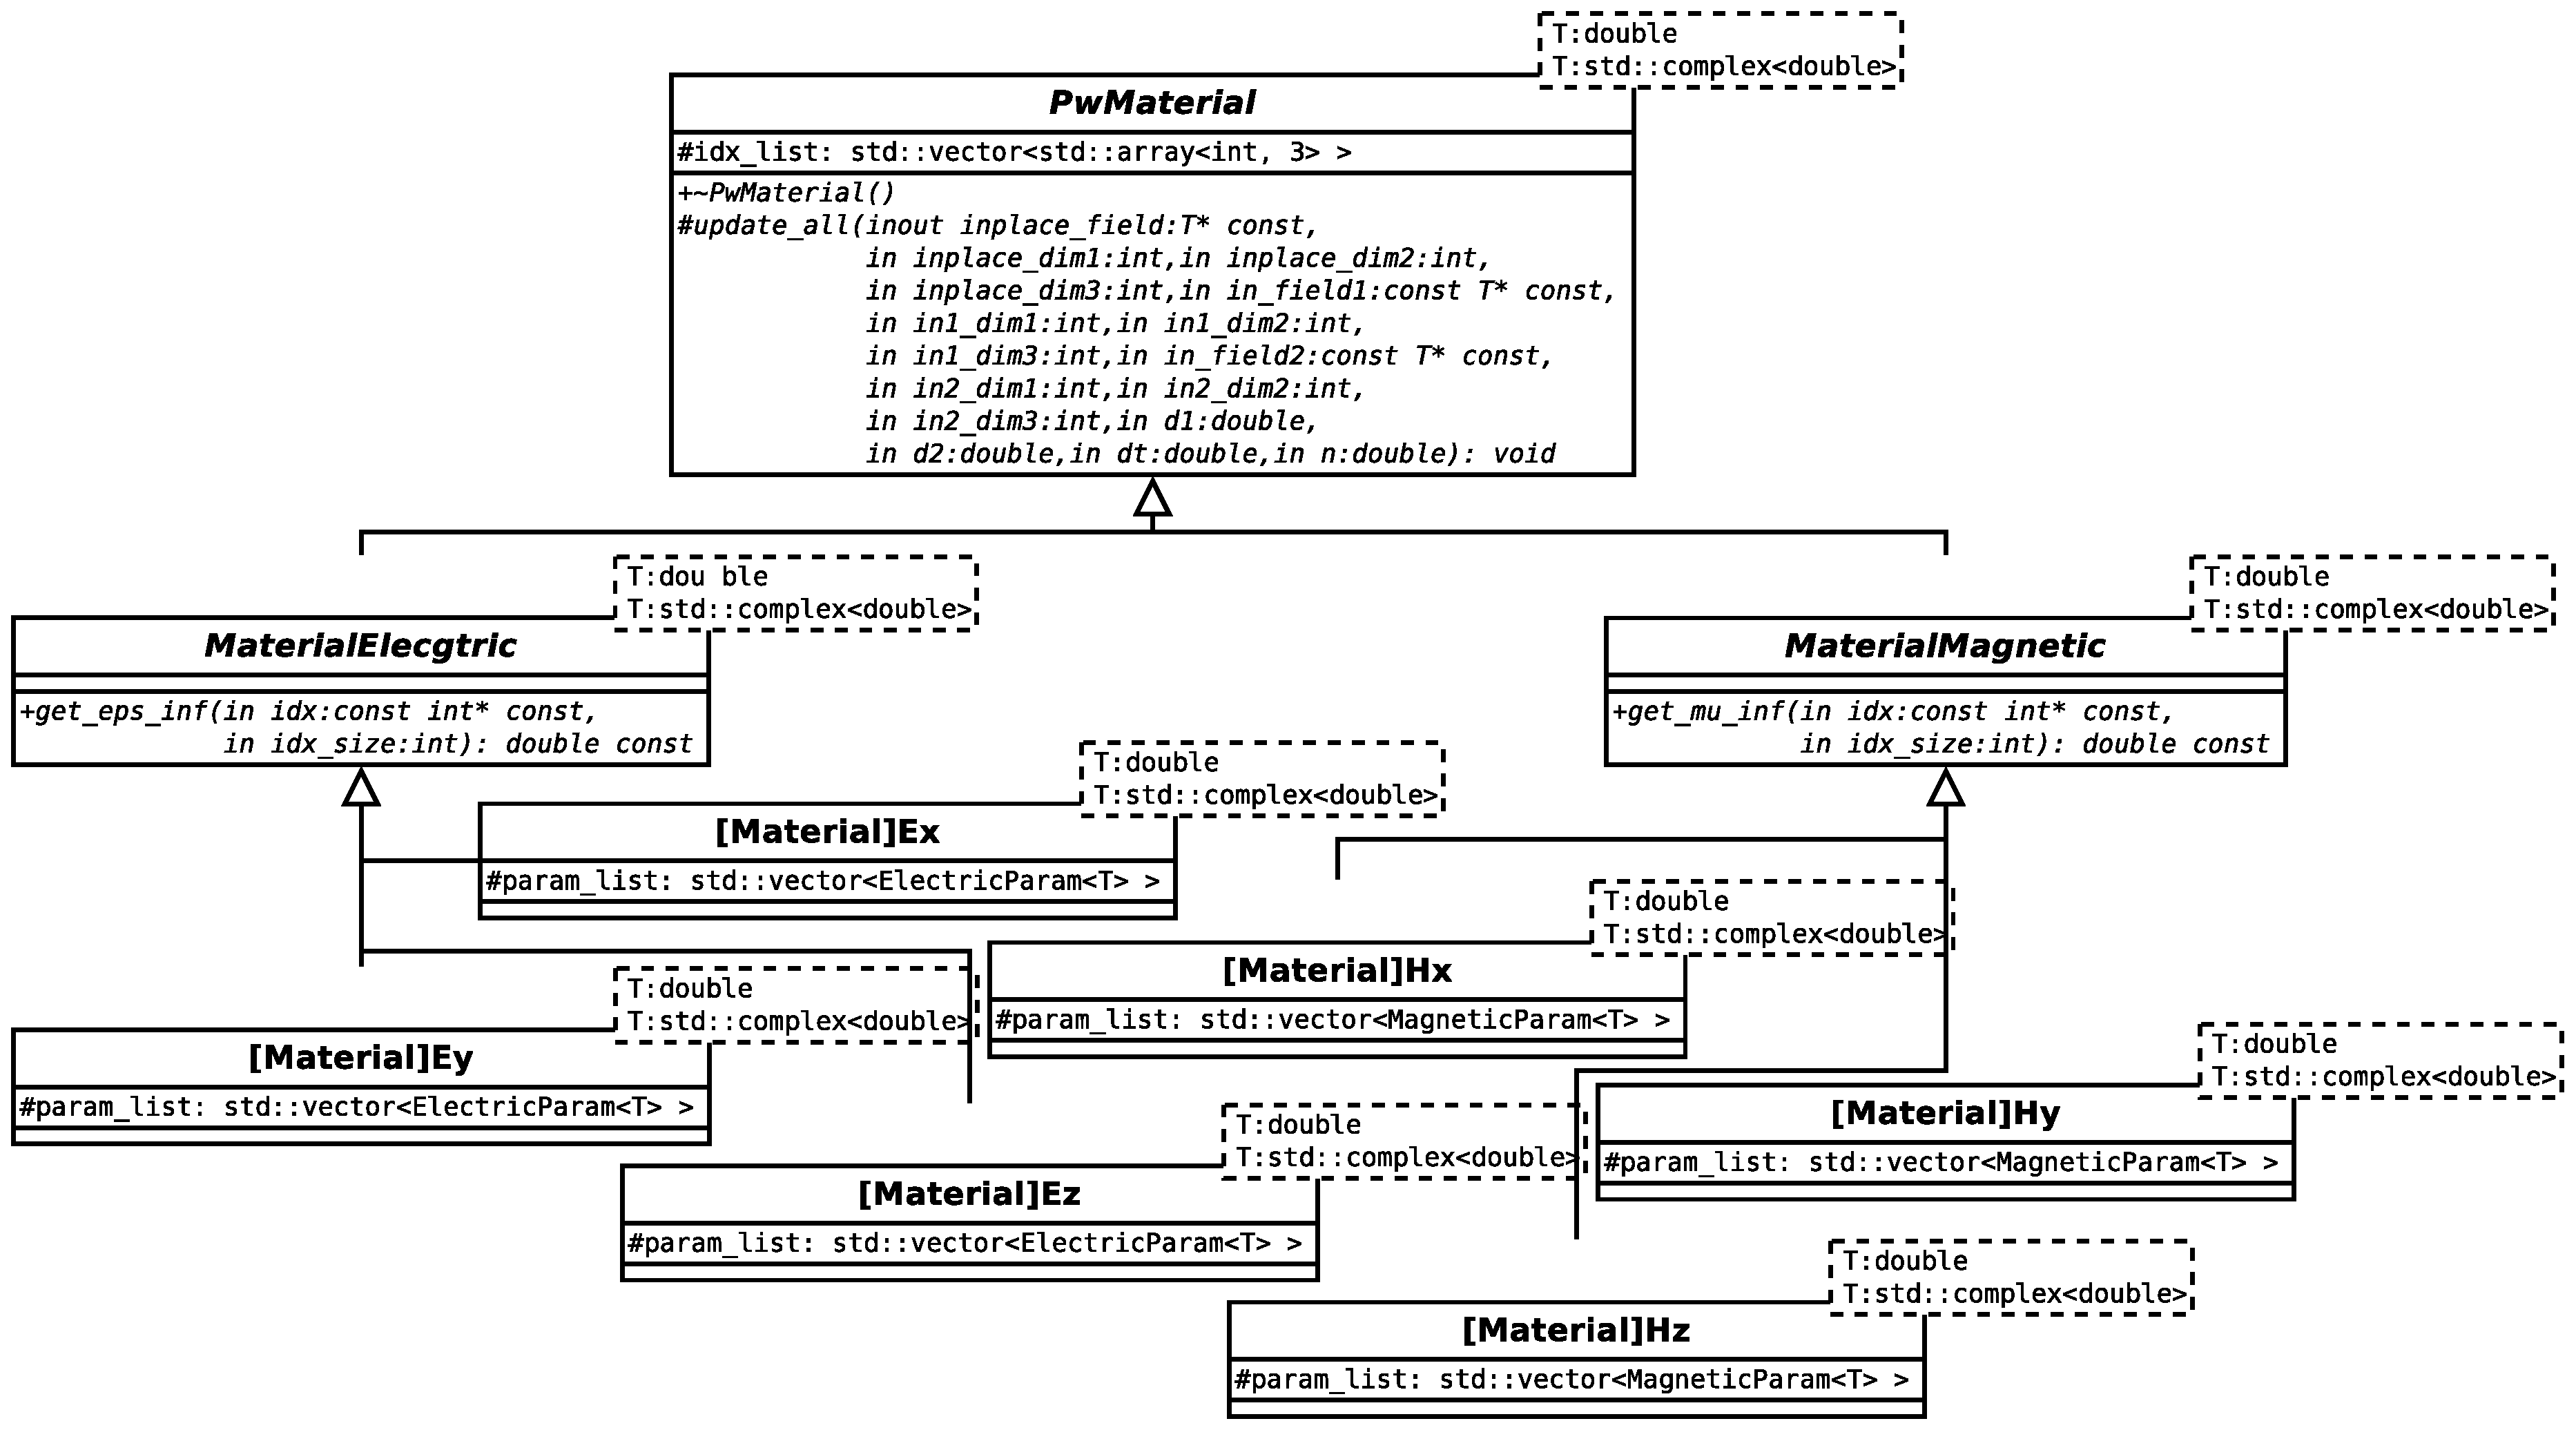
\includegraphics[keepaspectratio,width=1\textwidth]{figure/pw_material}
  \caption{The UML class diagram (with only attributes and virtual methods) of the abstract base classes for the material representation in GMES\index{GMES}. GMES\index{GMES} provides abstract base classes: \texttt{MaterialElectric} and \texttt{MaterialMagnetic} for the electric and magnetic field updates, respectively. Users can define a new material by inheriting these classes and making them as a concrete class by defining an update method. Also, \texttt{ElectricParam} and \texttt{MagneticParam} classes store the parameters required for the update method.}
  \label{fig:pwmaterial}
\end{figure}

Instead of storing the material data in a single array for one parameter, the material data is spread over the material objects. This is possible due to the characteristic feature of the FDTD\index{FDTD} algorithm as mentioned above. The class structure of GMES\index{GMES} is shown in figure \ref{fig:pwmaterial}. GMES\index{GMES} provides a class named \texttt{PwMaterial}\index{PwMaterial class} which is updated by a \emph{piecewise} or in other words, a type-by-type update scheme\index{piecewise scheme}. All the materials that GMES\index{GMES} provide are derived from this abstract base class. This class is defined as a template and can handle electromagnetic fields with real and complex values that appear in the same code. The actual time-stepping algorithm is implemented in the following concrete classes: \texttt{[Material]\{Ex, Ey, Ez, Hx, Hy, Hz\}} where \texttt{[Material]} represents the name of the material or the type of the model used to represent the electric permittivity and magnetic permeability of the particular material, and  the names in \texttt{\{\}} represent the electric and magnetic fields. 

These concrete classes also store the list of parameter data objects instantiated by \texttt{ElectricParam<T>} and \texttt{MagneticParam<T>}. The way in which the lists of indices of the voxel\index{voxel} and parameter data objects are stored has a huge impact on the time-stepping speed of GMES\index{GMES}. The container to store the data should have a good unordered traversal performance, since it is iterated at every time-step. Furthermore, the container should also consume a minimum amount of memory space, even though the number of voxels\index{voxel} in FDTD\index{FDTD} is huge. A C\verb!++! standard container such as \texttt{std::vector} can fulfill these requirements. Additionally, \texttt{std::vector} provides a notable feature as well: a contiguous storage. Rather than storing pointers of the voxel\index{voxel} index and parameter data objects, GMES\index{GMES} stores instances of the voxel\index{voxel} index and parameter data objects in the \texttt{std::vector} to keep the data locality in memory. This contiguous storage which is independent of the order of indices and sequential access, reduces the memory access bottleneck by increasing the cache hit ratio. The index and \texttt{[Material]Param<T>} objects are stored in separate \texttt{std::vector}s since they are defined at different inheritance hierarchies as shown in figure \ref{fig:pwmaterial}. The \texttt{std::vector} which stores the parameter data objects can only be defined after the update function is implemented.

The OOP\index{OOP} design feature of GMES\index{GMES} has benefits in the implementation since the piecewise material classes can be written either in C\verb!++! or Python. Some classes of GMES\index{GMES}, especially the computationally loaded classes are implemented in C\verb!++!. These classes, however, have their base classes which can be concretized in Python, as well. This feature enables the user for a faster implementation, thereby allowing them to investigate and confirm any novel physical phenomena more rapidly than before. The user can also then convert the code into C\verb!++! for faster execution if desired.

\section{Supporting materials}
\label{sec:material}
GMES\index{GMES} provides the family of classes named \texttt{Material}\index{\texttt{Material} class}, used in the front-end to define materials and structures of a target device, in a separate manner to those of \texttt{PwMaterial} classes\index{\texttt{PwMaterial} class} that are used internally for time-stepping. The material classes have been designed to support (an)isotropic, (non-)linear, and (non-)dispersive materials, however, the current version does not have any non-linear material implementation yet. Probably, the most basic material class used in real-world simulation is the \texttt{Dielectric} class\index{\texttt{Dielectric} class}, which represents isotropic, linear, and non-dispersive dielectric materials.

The isotropic linear dispersive materials are modeled using various models such as Debye\index{Debye theory}, Drude\index{Drude theory}, Lorentz\index{Lorentz theory}, and the critical point theory\index{critical point theory} \cite{ashcroft_solid_1976, etchegoin_elasto-optical_1993}. The Drude and Lorentz models are provided in \texttt{Drude}\index{\texttt{Drude} class} and \texttt{Lorentz} classes\index{\texttt{Lorentz} class}, respectively, which are implemented by using the auxiliary differential equation method\index{auxiliary differential equation method} (ADE\index{ADE method}) \cite{okoniewski_drude_2006, okoniewski_simple_1997}. The poles for these classes are supported by passing a tuple of \texttt{DrudePole} and \texttt{LorentzPole}\index{\texttt{LorentzPole} class}, respectively. Here, the classes, \texttt{DrudePole}\index{\texttt{DrudePole} class} and \texttt{LorentzPole}\index{\texttt{LorentzPole} class}, contain the parameters required for realizing Drude\index{Drude model} and Lorentz models\index{Lorentz model}, respectively. For better representation of the dispersive property of noble metals, GMES\index{GMES} also provides the ADE\index{ADE method} and piecewise-linear recursive-convolution\index{piecewise-linear recursive-convolution method} (PLRC\index{PLRC method}) implementation of the Drude-critical point (DCP\index{DCP}) model\index{Drude-critical point model} \cite{prokopeva_optical_2011} in \texttt{DcpAde}\index{\texttt{DcpAde} class} and \texttt{DcpPlrc} classes\index{\texttt{DcpPlrc} class}, respectively. These classes also support multiple poles by passing tuples of \texttt{DrudePole}\index{\texttt{DrudePole} class} and \texttt{CriticalPoint}\index{\texttt{CriticalPoint} class}. In particular, DCP\index{DC} models are useful to accurately describe the electrical permittivity of metals accounting for the interband transition\index{interband transition}. A typical example for representing silver using the \texttt{DcpPlrc} class\index{\texttt{DcpPlrc} class} is shown in figure \ref{fig:silver}.

\begin{figure}[Hp!]
  \centering
  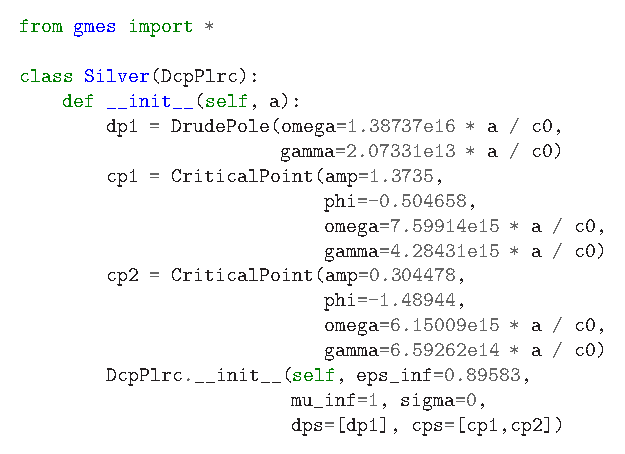
\includegraphics[keepaspectratio=true]{figure/silver}
  \caption{An example of defining a new material using DCP model. This class represents the electric permittivity of silver in the wavelength range from 200 nm to 1000 nm. The parameters used in the code were obtained from tabulated values available in \citet{johnson_optical_1972} by fitting.}
  \label{fig:silver}
\end{figure}

GMES\index{GMES} also supports the ABC\index{ABC} by providing an absorbing material which encapsulates the structure. GMES\index{GMES} has two separate implementations of the ABC\index{ABC}. One is the ADE\index{ADE method} implementation of the uniaxial perfectly matching layer\index{uniaxial perfectly matching layer} (UPML\index{UPML}), which represents the PML\index{PML} as a uniaxial medium \cite{gedney_anisotropic_1996}, and is represented by \texttt{Upml} class\index{\texttt{Upml} class}. The other class is \texttt{Cpml}\index{\texttt{Cpml} class}, a recursive convolution\index{recursive convolution} (RC\index{RC}) implementation of the complex-frequency-shifted PML\index{complex-frequency-shifted PML} (CFS-PML\index{CFS-PML}) \cite{roden_convolution_2000}. Though the current version of GMES\index{GMES} has two individual implementations of the ABC\index{ABC}, the \texttt{Upml} class\index{\texttt{Upml} class} will be deprecated since UPML\index{UPML} is a restricted form of CFS-PML\index{CFS-PML} \cite{taflove_computational_2005}. GMES\index{GMES} has other material classes to be used internally: \texttt{Dummy} and \texttt{Const}. \texttt{Dummy}\index{\texttt{Dummy} class} does nothing in the update method, and is only used to terminate the Yee grid\index{Yee grid} at certain boundaries. \texttt{Const}\index{\texttt{Const} class} sets the electromagnetic field to a given value, and was developed for debugging.

\section{Boundary conditions}
\label{sec:boundary}
The boundary condition of GMES\index{GMES} is based on the Cartesian logical process topology\index{Cartesian topology} with message passing interface\index{message passing interface} (MPI\index{MPI}) \cite{message_passing_interface_forum_mpi:_2009}. MPI\index{MPI} enables GMES\index{GMES} to undertake distributed-memory computing, thereby it can divide and distribute very large problems on multiple processes. Whether GMES\index{GMES} divides the whole calculation domain into chunks or not, the boundaries of the calculation domains are always synchronized with the adjacent boundaries that are represented in the Cartesian topology\index{Cartesian topology}. 

Figure \ref{fig:yee_cell} shows the voxel\index{voxel} index of a Yee cell used in GMES\index{GMES}. The black circles and squares represent the voxel\index{voxel} for the electric and magnetic field, respectively, and belong to the Yee cell\index{Yee cell} under consideration. Similarly, the orange circles and purple squares represent the voxel\index{voxel} for the electric and magnetic field, respectively, but in this case belong to the adjacent cells of the Yee cell\index{Yee cell} under consideration. 

\begin{figure}[hp!]
  \begin{center}
    \subfigure[The voxel index of each electromagnetic field component in a Yee cell]{
      \includegraphics[keepaspectratio,width=0.45\textwidth]{figure/yee_cell}
      \label{fig:yee_cell}
    }
    \subfigure[Synchronization of the field values in Cartesian topology]{
      \includegraphics[keepaspectratio,width=0.45\textwidth]{figure/cartesian_topology}
      \label{fig:cartesian_topology}
    }
  \end{center}
  \caption{(a) Black circles and squares are respectively the electric and magnetic field arrays that belong to the Yee cell. Orange circles and purple squares are the buffers for the electric and magnetic fields, respectively. (b) The buffers are filled with the values from the opposite side, and are used to update the outermost electromagnetic fields. The numbers in the parentheses are the coordinates in the Cartesian topology, and the direction of arrows represents the direction in which the field data is copied.}
  \label{fig:yee_cell_and_topology}
\end{figure}

Consider for example the $z$ component of the electric field of the voxel\index{voxel}, i.e. \texttt{ez[i,j,k]}. This voxel\index{voxel} belongs to the Yee cell\index{Yee cell} under consideration. To evaluate \texttt{ez[i,j,k]}, we require the values of magnetic fields of the adjacent cells, i.e. \texttt{hx[i,j,k+1]} and \texttt{hy[i,j,k+1]}. If the Yee cell is situated at the boundary, then \texttt{hx[i,j,k+1]} and \texttt{hy[i,j,k+1]} may not have immediate values, and are updated by the \texttt{Dummy}\index{\texttt{Dummy} class} objects, and hence the values will be copied from the voxels\index{voxel} situated at the boundary touching it. If not, \texttt{hx[i,j,k+1]} and \texttt{hy[i,j,k+1]} belong to adjacent Yee cells, and the field values of the voxels\index{voxel} will be updated by the corresponding Yee cell to which the voxels\index{voxel} belong.

If a Bloch wave vector\index{Bloch wave vector} is provided by the user, the synchronization procedure of GMES\index{GMES} would adopt a periodic boundary condition\index{periodic boundary condition} \cite{joannopoulos_photonic_2008}. The synchronization scheme adopted in GMES\index{GMES} for the electric and magnetic fields is depicted in figure \ref{fig:cartesian_topology}. During the synchronization procedure, GMES\index{GMES} then uses complex values for the electromagnetic fields, and the fields are multiplied by a phase shift term given by $\exp(i k_i \Lambda_i)$ where $k_i$ ($i=x,y,z$) is the directional component of the Bloch wave vector\index{Bloch wave vector} and $\Lambda_i$ is the physical distance between the source and destination voxel\index{voxel}. The distance between the boundaries `b' and `c' is 0, and hence the phase term is 1 when the fields are passed between them. When the fields are passed between the boundaries `a' and `d', the fields are multiplied by $\exp(i k_i \Lambda_i)$ since $\Lambda_i$ is not 0.

\section{Input source excitations}
\label{sec:source}
GMES\index{GMES} supports various source excitations as the input. The piecewise updating scheme\index{piecewise updating scheme} which was used for material implementation, was successfully adopted for the implementation of excitation sources. Using \texttt{PwSource}\index{\texttt{PwSource} class} and \texttt{PwSourceParam}\index{\texttt{PwSourceParam} class} as the base classes, source classes were defined whose hierarchy is shown in figure \ref{fig:pwsource}.

\begin{figure}[hp!]
  \centering
  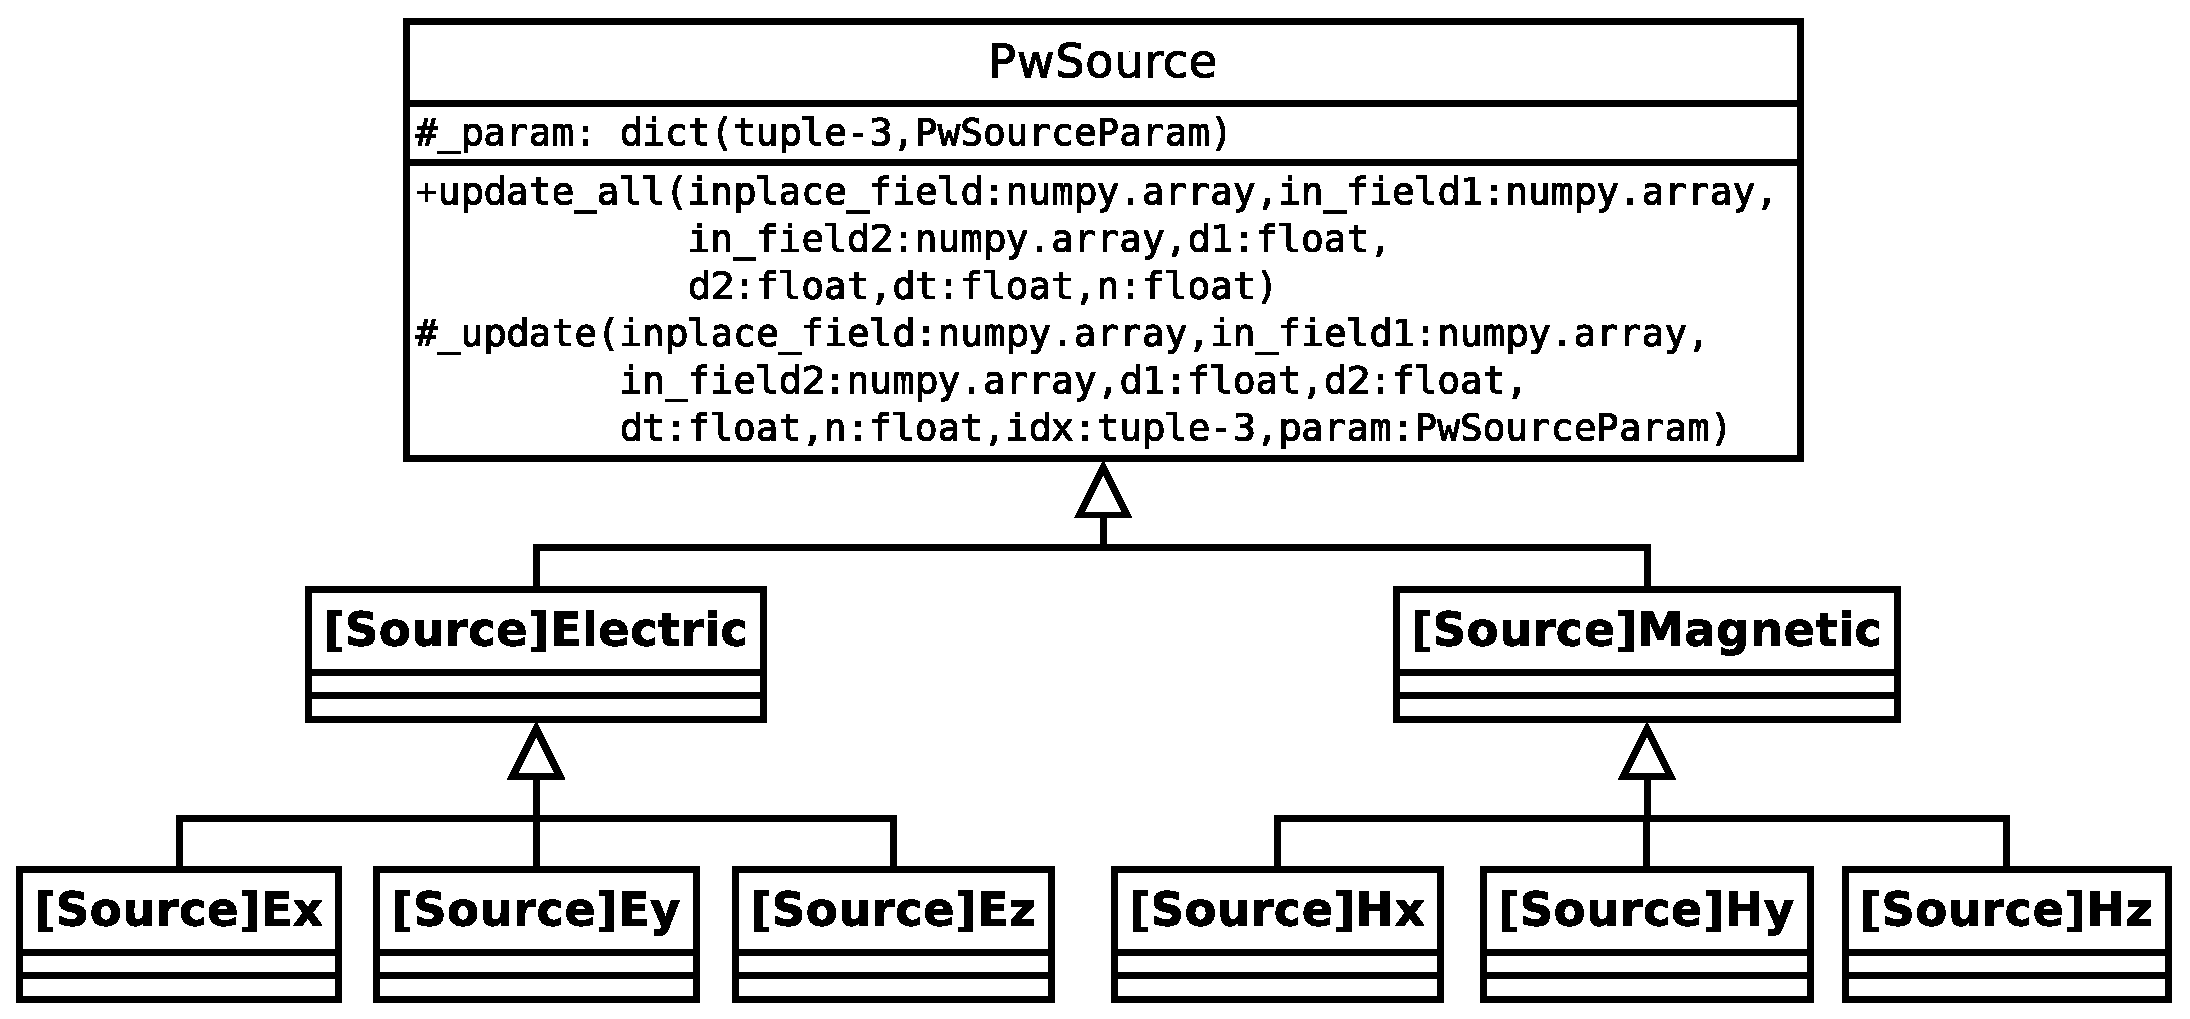
\includegraphics[keepaspectratio,width=\textwidth]{figure/pw_source}
  \caption{The UML class diagram (with only selected attributes and methods) of the abstract base classes for the source representations in GMES\index{GMES}. GMES\index{GMES} provides an abstract base class, \texttt{PwSource}. The class \texttt{PwSourceParam}  stores the parameters required for the update method. Users can define a new source by inheriting these classes and making them as a concrete class by defining an update method.}
  \label{fig:pwsource}
\end{figure}

This design was based on the following two criteria. First, the number of voxels\index{voxel} occupied by the input source is small compared to the number of voxels\index{voxel} in the entire computation domain. Thus, the computational burden due to \texttt{PwSource} during time-stepping is not significant. 

Second, for implementing transparent sources (for eg, total-field/scattered-field\index{total-field/scattered-field source} (TF/SF\index{TF/SF source}), Gaussian beam source\index{Gaussian beam source}), an auxiliary one-dimensional FDTD\index{FDTD} has to be executed for the generation of a look-up table for the space-time variation of the incident field \cite{merewether_implementing_1980,mur_absorbing_1981,umashankar_novel_1982}. As a result, the \texttt{PwSource}\index{\texttt{PwSource} class} needs to access the Python layer of GMES\index{GMES} for the execution. Therefore, it is legitimate to implement \texttt{PwSource}\index{\texttt{PwSource} class} in Python rather than in C\verb!++!.  

\begin{figure}[hp!]
  \centering
  \includegraphics[width=0.7\textwidth]{figure/tfsf_scheme}
  \caption{Schematics of the TF/SF source mechanism}
  \label{fig:tfsf_scheme}
\end{figure}

The spatial properties of input sources in GMES\index{GMES} are defined using the \texttt{Src} class\index{\texttt{Src} class}. A point source is supported by a class named \texttt{PointSource}\index{\texttt{PointSource} class}. The user can set the $\mathbf E$, $\mathbf H$, $\mathbf J$, and $\mathbf M$ sources at a specific location. The plane-wave source is provided by the \texttt{TotalFieldScatteredField} class\index{\texttt{TotalFieldScatteredField} class}, an implementation of the TF/SF technique\index{TF/SF source} with a matched numerical dispersion technique \cite{guiffaut_perfect_2000} which provides dispersion compensation. Also, if a user wants to use a beam source whose intensity is concentrated in the vicinity of the propagating axis, the \texttt{GaussianBeam} class\index{\texttt{GaussianBeam} class} can be a good choice. 

%% \begin{figure}[hp!]
%%   \centering
%%   \includegraphics[width=\textwidth]{figure/gaussian_beam_scheme}
%%   \caption{Schematics of the Gaussian beam source mechanism}
%%   \label{fig:gaussian_beam_scheme}
%% \end{figure}

Time-varying features such as frequency, and amplitude of the envelope of the sources described above is set by the \texttt{SrcTime} class\index{SrcTime class}. The current version of GMES\index{GMES} provides three classes for time-varying oscillators. The first one is the \texttt{Continuous} class\index{\texttt{Continuous} class} which generates a sinusoidal oscillation with a constant amplitude. The second is the \texttt{Bandpass} class\index{\texttt{Bandpass} class} which provides a Gaussian pulse\index{Gaussian pulse} with a given bandwidth. The last one is the \texttt{DifferentiatedGaussian} class\index{\texttt{DifferentiatedGaussian} class} which generates a differentiated Gaussian pulse\index{differentiated Gaussian pulse}.

\section{User interface and scripting}
\label{sec:interface}
A GMES\index{GMES} script can be passed to a Python interpreter or typed line-by-line in a Python interpreter\index{Python interpreter}. figure \ref{fig:metal_array} shows a simple example of a plasmon waveguide situated in vacuum which consists of six silver spherical nanoparticles of radius 25 nm. The distance between the centers of adjacent nanoparticles is 75 nm.

\begin{figure}[hp!]
  \begin{center}
    \subfigure[A simple Python code using GMES, for the simulation of a plasmon waveguide consisting of an array of six silver nanoparticles.]{
      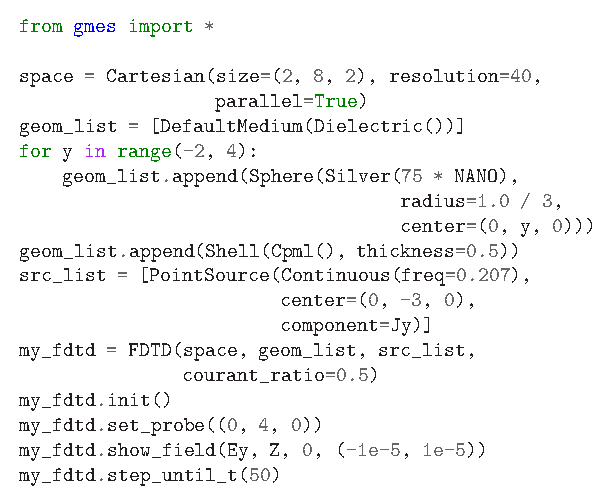
\includegraphics[keepaspectratio]{figure/metal_array_code}
      \label{fig:metal_array_code}
    }
    \subfigure[The distribution of the $y$ component electric field ($E_y$)]{
      \includegraphics[keepaspectratio,width=\textwidth]{figure/metal_array_field}
      \label{fig:metal_array_field}
    }
  \end{center}
  \caption{(a) A simple GMES example showing a plasmon waveguide. The definition of \texttt{Silver} class used in this example was described in figure \ref{fig:silver}. (b) The $E_y$ field display showing the propagation of the longitudinal mode of the plasmon waveguide. This figure is a combination of three displays obtained from three processes.}
  \label{fig:metal_array}
\end{figure}

A GMES\index{GMES} script starts with the package import statement like any other ordinary Python packages. The first line which follows the import statement is to define the calculation coordinate. The current version of GMES\index{GMES} supports only the \index{Cartesian} coordinates, which can be defined by the \texttt{Cartesian} class\index{\texttt{Cartesian} class} with a given size and resolution. If a user wants to execute GMES\index{GMES} on a distributed memory environment, the option \texttt{parallel} should be set to \texttt{True} and the script should be executed using a MPI enabled Python interpreter\index{MPI enabled Python interpreter} \cite{dalcin_mpi_2012}. GMES\index{GMES} uses dimensionless units\index{unit}; thus users can set any length scale for the unit size of Cartesian coordinates. Though GMES\index{GMES} does not have a graphical user interface\index{graphical user interface} (GUI\index{GUI}), it provides a simple CAD\index{CAD} facility similar to libctl\index{libctl} \cite{johnson_libctl_2012}. This enables users to define customized structures in GMES\index{GMES}. 

The geometrical structures are defined as a list of geometric primitives. The first elements of the list should be a \texttt{DefaultMedium} which fills the whole calculation domain with a given material. We can fill the geometric primitives with a predefined material. In the example demonstrated in figure \ref{fig:metal_array}, we filled the calculation domain with a dielectric material having an electrical permittivity and magnetic permeability of 1. With the dimensionless unit scheme of GMES\index{GMES}, the electrical permittivity of vacuum ($\epsilon_0$) and magnetic permeability of vacuum ($\mu_0$) are set as 1. In GMES\index{GMES}, therefore, electric permittivity ($\epsilon$) and magnetic permeability ($\mu$) are the same as relative electrical permittivity ($\epsilon_r$) and magnetic permeability ($\mu_r$) of the material. The geometrical positions of all objects are determined by the relative position from the center of the calculation domain which is always set to $(0,0,0)$. 

GMES\index{GMES} determines the material at a voxel\index{voxel} by referencing a geometry list (\texttt{geom\_list} shown in figure \ref{fig:metal_array_code}). A backward search of the list is performed where GMES\index{GMES} searches for the structure containing the voxel\index{voxel}, and when a match is found, GMES\index{GMES} takes the first structure which contains the voxel\index{voxel}. It should be noted that a match is always found since the \texttt{DefaultMedium} class which is one of the structure primitives extends to infinity. The whole calculation domain is padded with \texttt{Shell} primitives to simulate an open space. 

In the code shown in figure \ref{fig:metal_array_code}, for example, the voxel\index{voxel} at $(0,-2,0)$ belongs to \texttt{DefaultMedium} and the \texttt{Sphere} centered at $(0,-2,0)$ of radius $1/3$. However, during the backward search, the first structure having the match is the \texttt{Sphere}, hence the material of the voxel\index{voxel} is determined to be \texttt{Silver} which fills the \texttt{Sphere}.

The input sources in GMES\index{GMES} are set as a separate list. An electric current source with certain frequency at a certain location can be set using the \texttt{PointSource} class. According to the unit system of GMES\index{GMES}, the unit of frequency is $c/a$, where $a$ is the characteristic length of the system.

GMES\index{GMES} provides several variants of the \texttt{FDTD\index{FDTD}} instance. This example uses an instance for the full three-dimensional simulation, \texttt{FDTD\index{FDTD}}, which uses all three components of the electric and magnetic fields each. If the electromagnetic field to be excited and the modeled geometry to be simulated has no variation in any of the axes, we can then reduce the use of memory and computational resources by using one of the following variants of the \texttt{FDTD\index{FDTD}} class: \texttt{TE\{x,y,z\}FDTD\index{FDTD}}, \texttt{TM\{x,y,z\}FDTD\index{FDTD}} or \texttt{TEM\{x,y,z\}FDTD\index{FDTD}}.

\texttt{FDTD\index{FDTD}} and its descendant classes provide utility functions to display or write out the electromagnetic fields and the distribution of the electric permittivity and magnetic permeability of the materials. Also, GMES\index{GMES} provides methods to control the time-stepping of the FDTD\index{FDTD} algorithm. If required, the time-stepping can be progressed for only one time-step or can be continued until a specified time is reached. For the example shown in figure \ref{fig:metal_array_code}, the computation is proceeding till a specified time of 150 ($a/c$).

In the example given, the user accesses the electromagnetic field by using an interface (\texttt{FDTD\index{FDTD}.\{set\_probe,show\_field\}}), however, the user can access the fields directly as well. Since GMES\index{GMES} uses NumPy arrays to store the electric and magnetic fields, the users can apply any operations of NumPy arrays\index{NumPy array} \cite{oliphant_guide_2006} on the stored electromagnetic fields.

\section{Current limitations and future works}
\label{sec:limitation}
GMES\index{GMES} was designed with the aim of providing a flexible material representation and easy maintenance, rather than execution speed. Though we have adopted techniques to overcome the reduction in execution speed without sacrificing the design simplicity, the execution speed of GMES\index{GMES} is still relatively slower than that of other FDTD\index{FDTD} implementations.

Our piecewise update scheme has one more advantage with regard to the parallelism. A general FDTD\index{FDTD} program does not fit to the single-instruction multiple-data\index{single-instruction multiple-data} (SIMD\index{SIMD}) type of parallelism, since each type of material has a different update method (i.e. instruction). The voxels\index{voxel} in a general FDTD\index{FDTD} program are updated sequentially. As a result, at a given time-step, the update instructions only for a given voxel\index{voxel} are known. The time-stepping procedure has no means to predict the instructions that will be used for updating the following voxel\index{voxel}. As a result, a complete SIMD\index{SIMD} parallelism cannot be achieved. On the other hand, GMES\index{GMES} gathers at once the same type of material having the same update method, and calls the same update instruction for all the voxels\index{voxel} in the \texttt{PwMaterial} object\index{PwMaterial class}. Thus, enhanced performance through SIMD\index{SIMD} parallelism can be attained by using specialized devices, such as a general-purpose computing on GPU (GPGPU\index{GPGPU}) to each \texttt{PwMaterial} object\index{PwMaterial class}, though this feature is not implemented in the current version yet.

In section \ref{sec:boundary}, we described the design concept of GMES\index{GMES} for parallelism in distributed memory environment\index{distributed memory environment}. Even in a shared memory system\index{shared memory system}, the parallelism feature of GMES\index{GMES} can be applied. The update algorithm can concurrently operate on each component of the electric or magnetic field. This feature of FDTD\index{FDTD} provides an option for multithreading parallelism. Though GMES\index{GMES} can handle this parallelism, it is currently restricted since the current version of the standard Python interpreter (CPython) cannot execute the multiple thread concurrently owing to global interpreter lock\index{global interpreter lock} (GIL\index{GIL}) \cite{lutz_programming_2011}. Once GIL\index{GIL} is removed from CPython\index{CPython}, GMES\index{GMES} would be able to fully avail from the benefits of the multithreading\index{multithreading} parallelism.

\section{Conclusion}
\label{sec:conclusion}
We have described in this paper about GMES\index{GMES}, a Python package which solves Maxwell's equations\index{Maxwell's equations} using the FDTD\index{FDTD} method. The design of GMES\index{GMES} uses a complete \index{OOP} approach, thereby providing an FDTD\index{FDTD} code that is well structured and easy to understand for the users without compromising the simplicity and speed of the FDTD\index{FDTD} algorithm.

Instead of a conventional update scheme where the voxels\index{voxel} are updated in a sequential manner, GMES\index{GMES} has adopted a unique strategy where the voxels\index{voxel} are grouped and then updated according to its material type. This design feature could minimize the virtual calls as well as avoid the usage of conditionals, thereby maintaining the simplicity and speed of the FDTD\index{FDTD} implementation. 

GMES\index{GMES} is a free package and allows the users to add new features, without complicating the FDTD\index{FDTD} algorithm. It also  provides ample scope for the users to experiment and implement new physical phenomena and design problems related to electromagnetics. Various kinds of sources and boundary conditions can be handled and implemented in GMES\index{GMES} with ease. We anticipate that these features would help GMES\index{GMES} to find its acceptance among researchers who want to make new FDTD\index{FDTD} codes without sacrificing the simplicity and speed of FDTD\index{FDTD}.
